\section*{\textbf{2 - Normally distributed pseudo-random numbers} \hrule} 



\subsection*{\textbf{Question 2}}
\begin{quote}

\textbf{Problem}
\begin{quote}
Make plots of three Gaussian random fields, using $ n =-1$, $n= -2$ and $n= -3$. Give the plots a size of 1024. The axis should be in physical size. Choose a minimum physical size and explain how this impacts the maximum physical size, the minimum $k$ and maximum $k$.
\end{quote}

\textbf{Solution} 

\begin{quote}
The Gaussian fields are initial created in k-space by using Fourier shifted coordinates (i.e the zeroth wavenumber corresponds with the left top and not the center) and are then inverse Fourier transformed. The method in which a field is created in $k$-space consists of two steps. One, the shifted wavenumbers are used to create a matrix with complex numbers based on the power spectrum. Two, the matrix is given the correct hermitian symmetry. The first step is briefly explained in the code. The second step, how the matrix is given the correct symmetry, is described below. 
\\
\\
The matrix has the correct symmetry if the complex number created with wavenumbers  $k_{x_i}, k_{y_j}$ is equal to the conjugate of the complex number created with wavenumbers $-k_{x_i}, -k_{y_j}$.  Let $N$ be the size of the $N \times N$ matrix  created in step one and let $c_{i,j}$ be the value in cell $i,j$. The matrix then has the correct hermitian symmetry if the following three points hold, % obtain the correct symmetry the following points should hold.

\begin{enumerate}
\item[A] \textbf{First row}: The value of matrix cell $c_{0,j}$ should be equal to the complex conjugate of the value in cell $c_{0,N-j}$, for $ 0 < j< N$. If $N$ is even then  the  value in cell $c_{0,N/2}$ should be equal to its own conjugate (i.e this value should only have a real component, because it is created with $k_0$ and $k_{nyquist}$).
\item[B] \textbf{First column}: This point is similar to the first point. The value of matrix cell $c_{i,0}$ should be equal to the complex conjugate of the value in the cell $c_{N-i,0}$, for $0 < i < N$. If $N$ is even then the value in cell $c_{N/2,0}$ should be equal to its own conjugate (i.e this value should only have a real component, because it is created with $k_{nyquist}$ and $k_{0}$).
\item[C] \textbf{Inner matrix}: The value in cell $c_{i,j}$ should be equal to the complex conjugate in cell $c_{N-i,N-j}$ with $1 \leq i, j < N$. If the matrix is even then cell $c_{N/2,N/2}$ must be real, as it is created with $k_{nyquist}, k_{nyquist}$. %, of which its complex conjugate is equal to its self. %corresponds to the niquest matrix and must thereby be equal to its own complex conjugate.
\end{enumerate}
The code that uses these properties to give the matrix the correct symmetry can be found on the next page. 
\\

The minimum physical size, the size of 1 cell, is chosen to be $ 1$ Mpc. This immediately fixes the maximum physical size as the grid must be 1024 $\times$ 1024. The maximum physical size is thus $ 1$ Mpc $ \times $ 1024 = 1024 Mpc. The minimum $k$ and maximum $k$ are fixed by the minimum and maximum size,

\begin{align}
k_{min} &= \frac{2 \pi}{ ( N \times \text{min distance} )} = \frac{2 \pi }{\text{max distance}} \\
k_{max} &= k_{nyquist} = \frac{2 \pi N}{ 2 \times ( N \times \text{ min distance} )} = \frac{ \pi}{\text{min distance}}
\end{align}

An increase in minimum distance would thus result in a smaller value for $k_{min}$ and a smaller value of $k_{max}$.
\\

The code that creates the fields and gives them the correct symmetry, can as mentioned before, be found below. \textbf{Important} to point out is that the same random uniform variables have been Box-Muller transformed to create the fields for the different powers, $n = -1$, $n = -2$, $n = -3$. This was done to save computational time and has as consequence that the three created plots show the evolution of the fluctuations as function of the power $n$ (i.e the second plot and third plot show the same kind of structure, only with a different intensity).

\end{quote}
\newpage
\textbf{Code} \\
The code is split over two files. The first file contains the code for the plots and the second file contains the code for the helper functions. \\

\textbf{Code - Plots}
\begin{quote}
The code for the creation of the plots.
\lstinputlisting{./Code/assigment_2.py}

\end{quote}

\textbf{Code - Symmetry}
\begin{quote}
The code containing the functions to create the matrix and give it the correct
symmetry. Only part of this file is shown, the full file is shown in assignment 4.
\lstinputlisting[firstline=0,lastline=108]{./Code/mathlib/misc.py}
\end{quote}
\newpage

\textbf{Plots - Fields}
\begin{quote}

\begin{figure}[!ht]
\centering
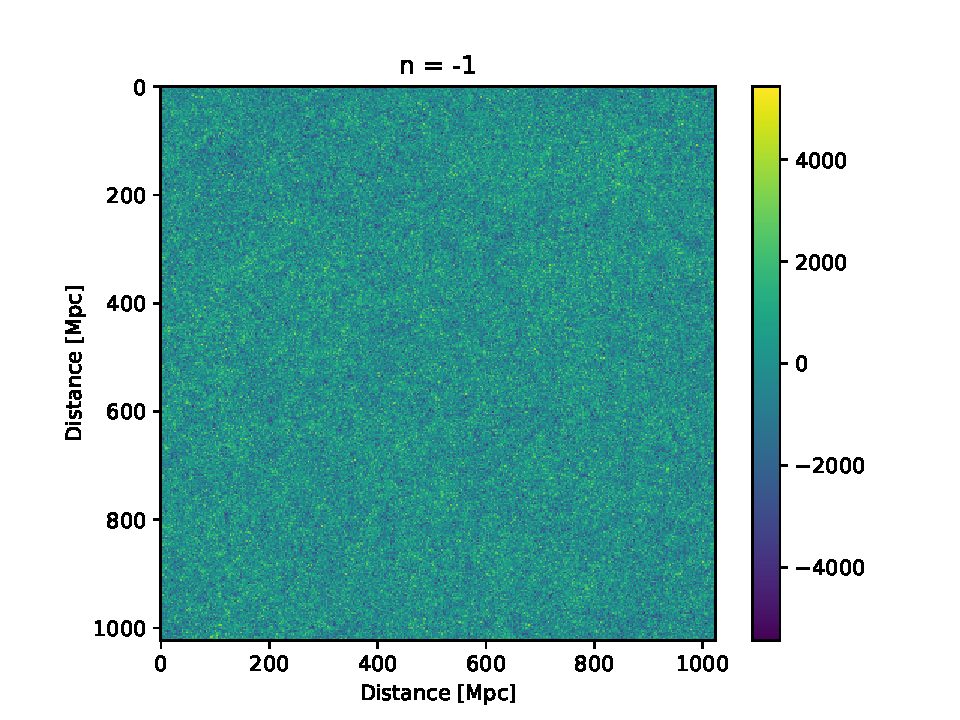
\includegraphics[width=14cm, height=9.5cm]{./Plots/2_field_-1.pdf}
\caption{The Gaussian field for $n = -1$ and a minimal physical size of 1 Mpc. The power drops for  $n = -1$ slowly, as result, mainly noise is expected. The plot seems to show that this is the case.}
\end{figure}

\begin{figure}[!ht]
\centering
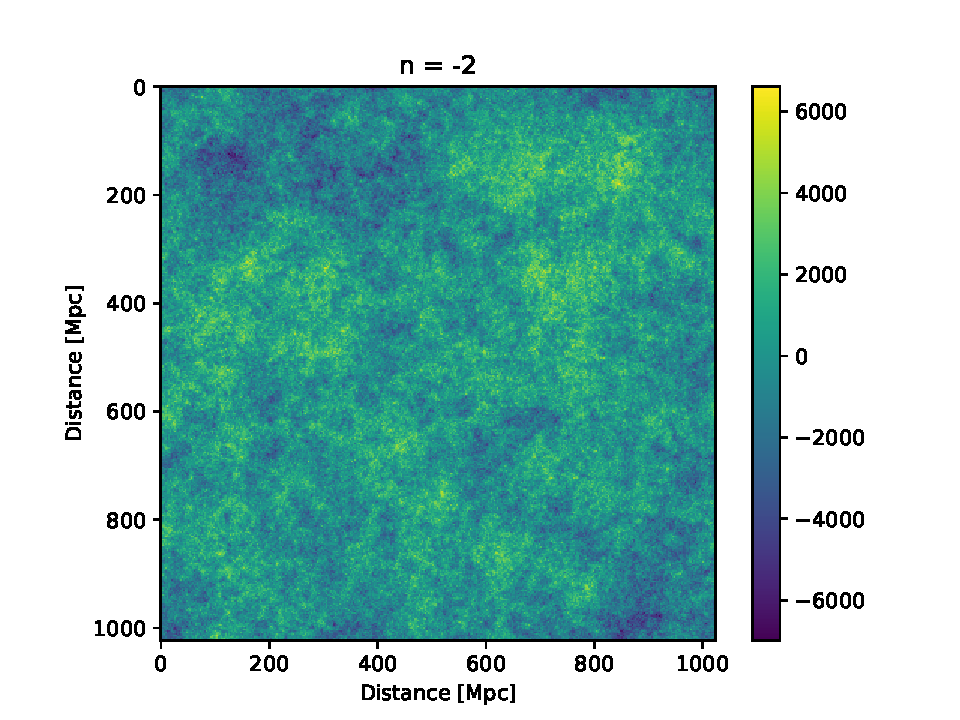
\includegraphics[width=14cm, height=9.5cm]{./Plots/2_field_-2.pdf}
\caption{The Gaussian field for $n = -2$ and a minimal physical size of 1 Mpc. The plot seems to be less noisy than the previous plot, which is expected as $n$ is now smaller.  }
\end{figure}
\end{quote}

\newpage
\begin{quote}

\begin{figure}[!ht]
\centering
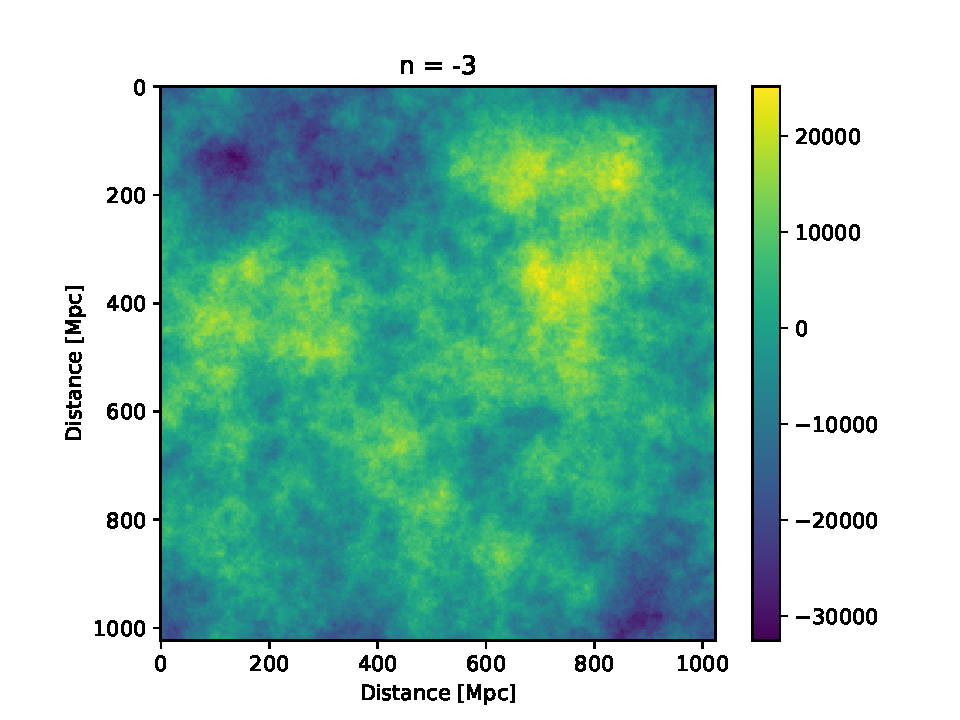
\includegraphics[width=14cm, height=9.5cm]{./Plots/2_field_-3.pdf}
\caption{The Gaussian field for $n = -3$ and a minimal physical size of 1 Mpc. High and low density fluctuations are now clearly visible. Notice that the plot looks similar to the plot for $n = -2 $. This is a consequence of using the same random uniform variables in the Box-Muller method. }
\end{figure}
\end{quote}



\end{quote}








